\chapter{Introducció}

Els expenedors automàtics de begudes fredes tenen una vida útil bastant llarga però les compres amb efectiu s'estan quedant enrere.

Cada dia el nombre de transaccions amb efectiu es van reduïnt. Els diners en efectiu ocupen espai i, sobretot les monedes, pesen molt. És per això que les transaccions s'encaminen cap al \textit{cashless} (en anglès, sense efectiu).


\begin{figure}
	\centering
	\begin{subfigure}[b]{0.45\textwidth}
		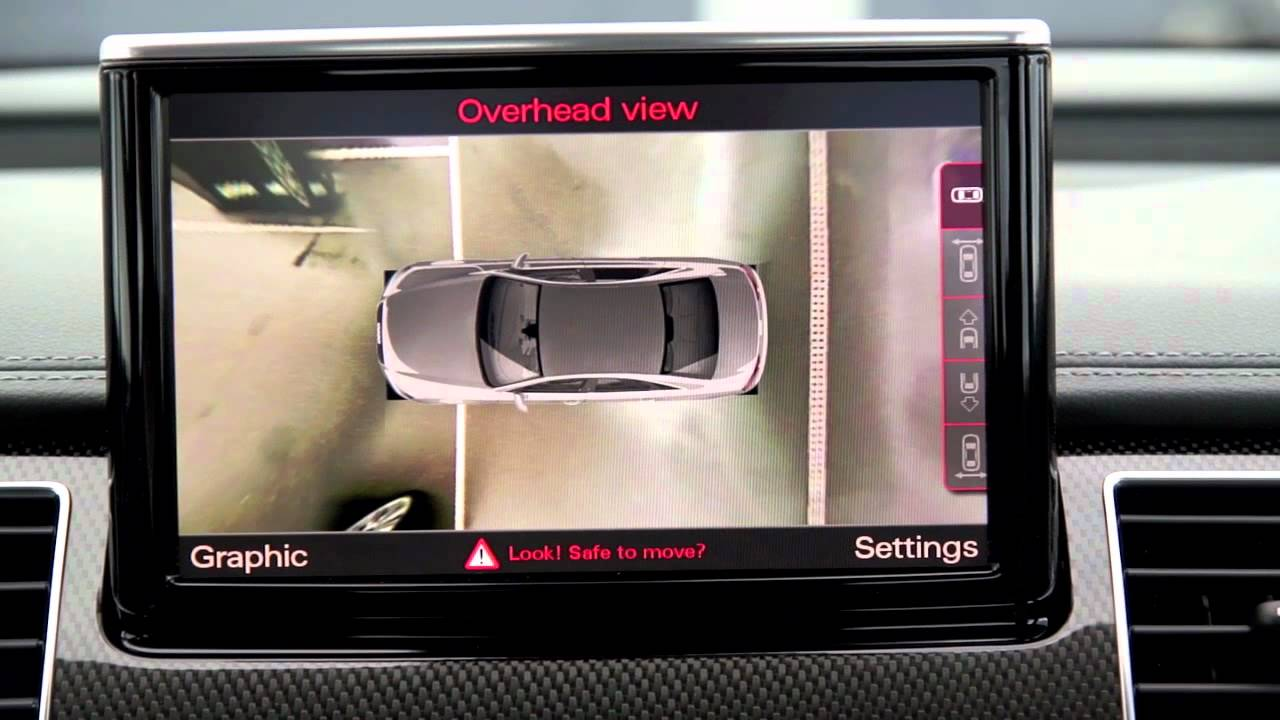
\includegraphics[width=\textwidth]{images/audi-intro}
		\caption{Audi S8 -- 360 View Camera}
		\label{fig:audi-intro-example}
	\end{subfigure}
	\hspace{0.5cm}
	\begin{subfigure}[b]{0.45\textwidth}
		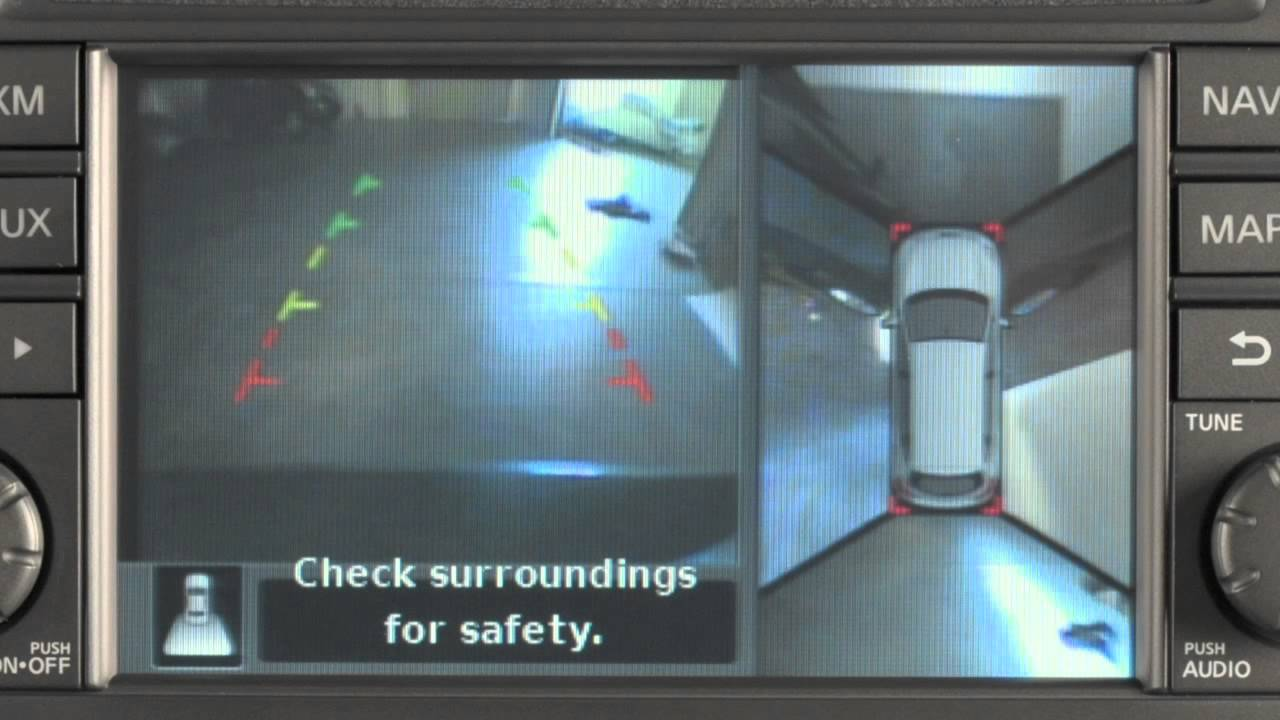
\includegraphics[width=\textwidth]{images/nissan-intro}
		\caption{Nissan Rogue -- Around View Monitor}
		\label{fig:nissan-intro-example}
	\end{subfigure}
	\caption{Two commercial 360\degree~vision systems display view}
	\label{fig:intro-example}
\end{figure}

\section{Objectius del projecte}

L'objectiu d'aquest projecte és dissenyar i desenvolupar un prototip per a un sistema \textit{cashless} que es pugui integrar dins d'expenedors automàtics existents. El projecte es centrarà en un model específic d'expenedor automàtic de begudes fredes (Dixie-Narco DNCB 386) perquè és l'expenedor que hi ha disponible per al desenvolupament.

Els principals objectius es poden resumir en els següents punts:

\vspace{-0.5em}
\begin{description}[font=\normalfont\textsl]
\item [Dissenyar i desenvolupar l'aplicació de servidor. ] El sistema de la solució serà un sistema centralitzat. Tot es gestionarà des d'un mateix lloc, i aquest serà l'aplicació de servidor.
\item [Dissenyar i desenvolupar l'aplicació de client. ] Per tal de poder controlar l'expenedor automàtic i comunicar-se amb l'aplicació de servidor, és necessaria l'aplicació de client.
\item [Dissenyar  Desenvolupar el sistema de hardware. ] Per tal de que l'aplicació de client pugui controlar l'expenedor, és necessari el sistema de hardware que farà d'interfície entre l'aplicació i els circuits de l'expenedor.
\end{description}

La feina feta durant aquests mesos s'ha centrat en desenvolupar el codi de les aplicacions i en desenvolupar el desplegament de hardware que s'integrarà a l'expenedor.

\section{Planificació del temps}

The time plan followed during this project development is shown in Figure~\ref{fig:gantt} Gantt Diagram. The developed work has been split in 8 work packages. A detailed description of each work package and the internal tasks developed can be found on Appendix~\ref{app:gantt}. 

\begin{figure}[ht]
\center
\begin{ganttchart}[
hgrid,
bar/.append style={fill=blue!50},
vgrid={*4{dotted},*1{dashed},*3{dotted},*1{dashed},*3{dotted},*1{dashed},*3{dotted},*1{dashed},*4{dotted},*1{dashed}},
x unit=0.47cm,
title height=1, 
y unit title=0.6cm,
y unit chart=0.8cm]{1}{22}
\gantttitle{Project timeline in months/weeks}{22} \\
\gantttitle{FEBR}{4}
\gantttitle{MARCH}{5}\gantttitle{APRIL}{4}\gantttitle{MAY}{4}\gantttitle{JUNE}{5} \\
\gantttitle[title label node/.append style={below left=-8pt and -7pt}]{\footnotesize\textit{Week}\quad1}{1}
\gantttitlelist
{2,...,22}{1} \\ 
\ganttbar{Training}{1}{6} \\
\ganttbar{System Design}{5}{8}\\
\ganttbar{System Development}{9}{17} \\ 
\ganttbar{Test Unit Design}{18}{18}\\ 
\ganttbar{Test Unit Development}{19}{20}\\
\ganttbar{Writing}{21}{22}
\end{ganttchart}
\caption{Project Gantt Chart}
\label{fig:gantt}
\end{figure}








